\documentclass[]{llncs}
\title{A Formal Connection between Security Automata and JML Annotations
\thanks{This work is partially funded by the IST FET
programme of the European Commission, under the IST-2005-015905
\textsf{Mobius} project.}}

\author{Marieke Huisman\inst{1} \and Alejandro Tamalet\inst{2}\thanks{Research done while at INRIA Sophia Antipolis}}
\institute{INRIA Sophia Antipolis, France \and
University of Nijmegen, Netherlands}


\usepackage{amsmath}
\usepackage{amssymb}
\usepackage{bbold}
\usepackage{epsfig}
\usepackage{psfrag}
\pagestyle{plain}
\usepackage{xspace}
\newcommand{\MVA}{\ensuremath{\mathit{MVA}}\xspace}

\newcommand{\name}{\ensuremath{\mathsf{name}}\xspace}
\newcommand{\clname}{\ensuremath{\mathsf{clname}}\xspace}
\newcommand{\mname}{\ensuremath{\mathsf{mname}}\xspace}
\newcommand{\cps}{\ensuremath{\mathsf{cps}}\xspace}
\newcommand{\init}{\ensuremath{\mathsf{init}}\xspace}
\newcommand{\evs}{\ensuremath{\mathsf{events}}\xspace}
\newcommand{\vdsA}{\ensuremath{\mathsf{mva\_var\_decl}}\xspace}
\newcommand{\vdsP}{\ensuremath{\mathsf{prog\_var\_decl}}\xspace}
\newcommand{\trans}{\ensuremath{\mathsf{trans}}\xspace}

\newcommand{\setof}[1]{\ensuremath{\mathcal{P}(#1)}}
\newcommand{\CP}{\ensuremath{\mathit{CP}}\xspace}
\newcommand{\EVENT}{\ensuremath{\mathit{Event}}\xspace}
\newcommand{\VarDeclA}{\ensuremath{\mathit{MVAVarDecl}}\xspace}
\newcommand{\VarDeclP}{\ensuremath{\mathit{ProgVarDecl}}\xspace}
\newcommand{\TRANS}{\ensuremath{\mathit{Trans}}\xspace}


\newcommand{\Name}{\ensuremath{\mathcal{N}}\xspace}
\newcommand{\type}{\ensuremath{\mathsf{type}}\xspace}
\newcommand{\Type}{\ensuremath{\mathcal{T}}\xspace}

\newcommand{\entry}{\ensuremath{\mathsf{entry}}\xspace}
\newcommand{\exit}{\ensuremath{\mathsf{exit}}\xspace}
\newcommand{\excexit}{\ensuremath{\mathsf{exc\_exit}}\xspace}
\newcommand{\etype}{\ensuremath{\mathsf{etype}}\xspace}


\newcommand{\Bool}{\ensuremath{\mathsf{Bool}}\xspace}
\newcommand{\Int}{\ensuremath{\mathsf{Int}}\xspace}
\newcommand{\Ref}{\ensuremath{\mathsf{Ref}}\xspace}
\newcommand{\Void}{\ensuremath{\mathsf{Void}}\xspace}

\newcommand{\B}{\ensuremath{\mathsf{B}}\xspace}
\newcommand{\I}{\ensuremath{\mathsf{I}}\xspace}
\newcommand{\R}{\ensuremath{\mathsf{R}}\xspace}
\newcommand{\Null}{\ensuremath{\mathsf{Null}}\xspace}
\newcommand{\One}{\ensuremath{\mathbb{1}}\xspace}

\newcommand{\Val}{\ensuremath{\mathcal{V}}\xspace}

\newcommand{\opr}{\ensuremath{\texttt{[\#\:}}}
\newcommand{\clr}{\ensuremath{\ \texttt{\#]}}}
\newcommand{\opri}{\ensuremath{\texttt{(\#\:}}}
\newcommand{\clri}{\ensuremath{\ \texttt{\#)}}}

\newcommand{\scp}{\ensuremath{\mathsf{source}}\xspace}
\newcommand{\tcp}{\ensuremath{\mathsf{dest}}\xspace}
\newcommand{\cp}{\ensuremath{\mathsf{current}}\xspace}
\newcommand{\event}{\ensuremath{\mathsf{event}}\xspace}
\newcommand{\guard}{\ensuremath{\mathsf{guard}}\xspace}
\newcommand{\action}{\ensuremath{\mathsf{action}}\xspace}

\newcommand{\target}{\ensuremath{\mathsf{target}}\xspace}
\newcommand{\expr}{\ensuremath{\mathsf{expr}}\xspace}

\newcommand{\listof}[1]{\ensuremath{\mathsf{list[}{#1}\mathsf{]}}\xspace}

\newcommand{\Store}{\ensuremath{\mathit{Store}}\xspace}
\newcommand{\Stmt}{\ensuremath{\mathit{Stmt}}\xspace}
\newcommand{\Expr}{\ensuremath{\mathit{Expr}}\xspace}

\newcommand{\Plus}{\ensuremath{\mathsf{Plus}}\xspace}
\newcommand{\EvalN}{\ensuremath{\mathsf{Eval_{\mathbb{N}}}\xspace}}
\newcommand{\EvalB}{\ensuremath{\mathsf{Eval_{\mathbb{B}}}\xspace}}
\newcommand{\EvalR}{\ensuremath{\mathsf{Eval_{\mathbb{R}}}\xspace}}
\newcommand{\EvalG}{\ensuremath{\mathsf{Eval_{\mathbb{G}}}\xspace}}

\newcommand{\NumExpr}{\ensuremath{\mathit{NumExpr}}\xspace}
\newcommand{\BoolExpr}{\ensuremath{\mathit{BoolExpr}}\xspace}
\newcommand{\RefExpr}{\ensuremath{\mathit{RefExpr}}\xspace}

\newcommand{\ttt}{\ensuremath{\mathsf{true}}\xspace}
\newcommand{\fff}{\ensuremath{\mathsf{false}}\xspace}

\newcommand{\Not}{\ensuremath{\mathsf{Not}}\xspace}
\newcommand{\Conj}{\ensuremath{\mathsf{And}}\xspace}
\newcommand{\GT}{\ensuremath{\mathsf{GT}}\xspace}
\newcommand{\Eq}{\ensuremath{\mathsf{Eq}}\xspace}

\newcommand{\Assign}{\ensuremath{\mathsf{Assign}}\xspace}
\newcommand{\BExpr}{\ensuremath{\mathsf{BExpr}}\xspace}
\newcommand{\CondExpr}{\ensuremath{\mathsf{CondExpr}}\xspace}
\newcommand{\Call}{\ensuremath{\mathsf{Call}}\xspace}
\newcommand{\NExpr}{\ensuremath{\mathsf{NExpr}}\xspace}
\newcommand{\RExpr}{\ensuremath{\mathsf{RExpr}}\xspace}

\newcommand{\CaseJML}{\ensuremath{\mathsf{CaseJML}}\xspace}
\newcommand{\IfThenElse}{\ensuremath{\mathsf{IfThenElse}}\xspace}
\newcommand{\Sequence}{\ensuremath{\mathsf{Sequence}}\xspace}
\newcommand{\Set}{\ensuremath{\mathsf{Set}}\xspace}
\newcommand{\Skip}{\ensuremath{\mathsf{Skip}}\xspace}
\newcommand{\StmtExpr}{\ensuremath{\mathsf{StmtExpr}}\xspace}
\newcommand{\Throw}{\ensuremath{\mathsf{Throw}}\xspace}
\newcommand{\TryCatch}{\ensuremath{\mathsf{TryCatch}}\xspace}
\newcommand{\While}{\ensuremath{\mathsf{While}}\xspace}
\newcommand{\Const}{\ensuremath{\mathsf{Const}}\xspace}
\newcommand{\Assert}{\ensuremath{\mathsf{Assert}}\xspace}

\newcommand{\Excpt}{\ensuremath{\mathcal{E}}}

\newcommand{\FieldDecl}{\ensuremath{\mathit{FieldDecl}}\xspace}
\newcommand{\ArgDecl}{\ensuremath{\mathit{ArgDecl}}\xspace}
\newcommand{\LocalVarDecl}{\ensuremath{\mathit{LocalVarDecl}}\xspace}
\newcommand{\GhostVarDecl}{\ensuremath{\mathit{GhostVarDecl}}\xspace}


\newcommand{\Program}{\ensuremath{\mathit{Program}}\xspace}
\newcommand{\Class}{\ensuremath{\mathit{Class}}\xspace}
\newcommand{\Method}{\ensuremath{\mathit{Method}}\xspace}

\newcommand{\param}{\ensuremath{\mathsf{param}}\xspace}
\newcommand{\pre}{\ensuremath{\mathsf{pre}}\xspace}
\newcommand{\post}{\ensuremath{\mathsf{post}}\xspace}
\newcommand{\lvars}{\ensuremath{\mathsf{lvars}}\xspace}
\newcommand{\body}{\ensuremath{\mathsf{body}}\xspace}
\newcommand{\preset}{\ensuremath{\mathsf{pre\_set}}\xspace}
\newcommand{\postset}{\ensuremath{\mathsf{post\_set}}\xspace}
\newcommand{\excset}{\ensuremath{\mathsf{exc\_set}}\xspace}
\newcommand{\res}{\ensuremath{\mathsf{res}}\xspace}
\newcommand{\restype}{\ensuremath{\mathsf{res\_type}}\xspace}
\newcommand{\super}{\ensuremath{\mathsf{super}}\xspace}
\newcommand{\inv}{\ensuremath{\mathsf{inv}}\xspace}
\newcommand{\ghostvars}{\ensuremath{\mathsf{ghost\_vars}}\xspace}
\newcommand{\fields}{\ensuremath{\mathsf{fields}}\xspace}
\newcommand{\methods}{\ensuremath{\mathsf{methods}}\xspace}

\newcommand{\classes}{\ensuremath{\mathsf{classes}}\xspace}

\newcommand{\Pstate}{\ensuremath{\mathit{PState}}\xspace}
\newcommand{\FullProgram}{\ensuremath{\mathit{FullProgram}}\xspace}
\newcommand{\Mprogram}{\ensuremath{\mathit{MProgram}}\xspace}
\newcommand{\FullState}{\ensuremath{\mathit{FullState}}\xspace}
\newcommand{\Astate}{\ensuremath{\mathit{AState}}\xspace}
\newcommand{\Mstate}{\ensuremath{\mathit{MState}}\xspace}
\newcommand{\MVAstate}{\ensuremath{\mathit{MVAState}}\xspace}
\newcommand{\pstate}{\ensuremath{\mathsf{pstate}}\xspace}
\newcommand{\progstate}{\ensuremath{\mathsf{prog\_state}}\xspace}
\newcommand{\program}{\ensuremath{\mathsf{program}}\xspace}
\newcommand{\PStore}{\ensuremath{\mathit{PStore}}\xspace}
\newcommand{\mva}{\ensuremath{\mathsf{mva}}\xspace}
\newcommand{\mvastate}{\ensuremath{\mathsf{mva\_state}}\xspace}
\newcommand{\ex}{\ensuremath{\mathsf{exc}}\xspace}
\newcommand{\st}{\ensuremath{\mathsf{store}}\xspace}
\newcommand{\stA}{\ensuremath{\mathsf{store_A}}\xspace}
\newcommand{\Excp}{\ensuremath{\mathit{Excp}}\xspace}
\newcommand{\Norm}{\ensuremath{\mathsf{Norm}}\xspace}
\newcommand{\Throwable}{\ensuremath{\mathsf{Throwable}}\xspace}
\newcommand{\NullPointer}{\ensuremath{\mathsf{RunTimeException}}\xspace}
\newcommand{\JMLExc}{\ensuremath{\mathsf{JMLException}}\xspace}
\newcommand{\fvs}{\ensuremath{\mathsf{fields}}\xspace}
\newcommand{\gvs}{\ensuremath{\mathsf{ghost\_vars}}\xspace}
\newcommand{\lvs}{\ensuremath{\mathsf{loc\_vars}}\xspace}

\newcommand{\exc}{\ensuremath{\mathit{exc}}\xspace}
\newcommand{\act}{\ensuremath{\mathit{act}}\xspace}

\newcommand{\etp}[2]{%
  P \vdash \langle #1 \rangle \triangleright \langle #2 \rangle}
\newcommand{\stp}[2]{%
  P \vdash \langle #1 \rangle \Rightarrow_P #2}

\newcommand{\gammain}{\ensuremath{\gamma_{\textsc{in}}}\xspace}
\newcommand{\gammanorm}{\ensuremath{\gamma_{\textsc{norm}}}\xspace}
\newcommand{\gammaexc}{\ensuremath{\gamma_{\textsc{exc}}}\xspace}

\newcommand{\deltaeval}{\ensuremath{\delta_{\textsc{eval}}}\xspace}
\newcommand{\deltaset}{\ensuremath{\delta_{\textsc{set}}}\xspace}
\newcommand{\deltacase}{\ensuremath{\delta_{\textsc{case}}}\xspace}
\newcommand{\deltaassert}{\ensuremath{\delta_{\textsc{assert}}}\xspace}

\newcommand{\md}{\ensuremath{\mathit{md}}\xspace}
\newcommand{\ev}{\ensuremath{\mathit{ev}}\xspace}
\newcommand{\invar}{\ensuremath{\mathit{inv}}\xspace}
\newcommand{\mn}{\ensuremath{\mathit{mn}}\xspace}
\newcommand{\with}{\ensuremath{\mathsf{\:with\:}}}
\newcommand{\id}{\ensuremath{\mathsf{id}}\xspace}


\newcommand{\br}[1]{\lbrack #1\rbrack}
\newcommand{\pif}[3]{\mathsf{if}\, #1\, \mathsf{then}\: #2\, \mathsf{else}\: #3}

\newcommand{\oldlvs}{\ensuremath{\mathit{old\_lvs}}\xspace}
\newcommand{\halted}{\ensuremath{\mathsf{halted}}\xspace}
\newcommand{\stuck}{\ensuremath{\mathsf{stuck}}\xspace}

\newcommand{\bp}{\ensuremath{\phantom{(}}}


\newcommand{\url}[1]{\texttt{#1}}

\newcommand{\marginnote}[1]{\marginpar{\mbox{#1}}}

\newcommand{\complete}{\ensuremath{\mathsf{complete}}\xspace}

\newcommand{\updatelvs}{\ensuremath{\mathsf{update\_lvs}}\xspace}
\newcommand{\lookupmthd}{\ensuremath{\mathsf{lookup\_mthd}}\xspace}
\newcommand{\lookupinv}{\ensuremath{\mathsf{lookup\_inv}}\xspace}

\usepackage{paralist}


\begin{document}

\maketitle
\begin{abstract}
Security automata are a convenient way to describe security
policies. They are often used to monitor an application, and to
interrupt execution as soon the security policy is violated. However,
run-time adherence checking is not always convenient.
Therefore, we consider the security automata as specification only,
\marginnote{\small AT: We don't verify adherence statically yet.}
% and verify adherence to it statically. We achieve this by generation
% of JML annotations that inline the monitor into the application.
and try to verify adherence to it statically. We want to achieve this by
generation of JML annotations that inline the monitor into the application.

% This paper describes the translation from security automata to program
% annotations, and proves that every translation step preserves the
% program behaviour.
% For this, we have developed a generic program semantics that is instantiated
% for monitoring and run-time annotation checking.
% Preservation of program behaviour boils down to a proof
% that monitoring will not find a security violation iff run-time
% annotation checking will not find any annotation violation (provided
% that earlier existing annotations are not violated either).
%
This paper describes the translation from security automata to program
annotations and proves preservation of program behaviour, which
boils down to a proof
that monitoring will not find a security violation iff run-time
checking the generated annotations will not find any violation.

%
% AT: This is future work.
% Once the program annotations are generated, an annotation propagation algorithm
% can be used to generate appropriate pre- and postconditions that
% are sufficient to guarantee adherence to the annotations, and that can
% be verified statically.
%
% Both program semantics, translation and correctness proofs are
% formalised using the PVS theorem prover. The correctness proofs
% revealed several subtleties that have to be considered in the
% definition of the algorithm and the program behaviour.
The correctness proofs are formalised using the PVS theorem prover.
They reveal several subtleties to be considered in the definition of the
algorithm and in the program requirements.
\end{abstract}


Java is a language commonly used on small device, with specific flavour
of it being used on heterogenous devices like cellphones or JavaCards. 
Thus taking into account their specific caracteristic each implementations
is important for verification.
Especially if specific system components change the overall behaviour of JVMs. 
Verification of system components is scattered through
litterature: there has been verifications of bytecode verifiers, as
well as access contoller. As far as our knowledge goes
though~\cite{HartelMoreau01}, the Security Manager of the JVM 
has not been verified and its semantic is not taken into
account when usually doing static verification of Java programs.


The main goal of this paper is to verify an implementation of a
Security Manager, and also to give a framework to more generally verify
programs taking into account the semantic differences that different
component of the JVM can bring to executions of program inside 
a JVM.

\vspace{-0.4cm}
\subsection{The Security Manager}
The Security Manager applies the security policies on two
levels. First on the library level: each time a writing or reading
operation is called for instance a call to the Security Manager is
made and if the caller has not respected a given security policy, a
{\tt SecurityException} is thrown.
Second on the JVM level: each time a class is
loaded, it checks on a meta level with the use of the ClassLoader
(which for this paper will be considered as a part of the JVM) if the
currently inspected class has the right to access a specified type
from an outside package.  
The latter is hard to take into account for a program verification, 
because it changes the behavior of type resolution which is part
of the language semantic.  A practical way to
model these changes would be to consider the Security Manager as an
Aspect which would weave at the cutting points representing type
resolution.
\vspace{-0.4cm}
\begin{figure}
\bcode
pa\=ckage a;\\
public class Main \{\+\\
  st\=atic \{\+\\
    Sy\=stem.setSecurityManager(new SecurityManager() \{\+\\
      pu\=blic void checkPackageAccess(String target) \{\+\\
        if\=(target.equals("b"))\\
          \>throw new SecurityException("That is true");\\
      \}\});\-\-\\
  \}\\
 \\
  public static void main(String[] args) \{\+\\
    System.out.println("Nextline will throw an exception");\\
    b.A a = new b.A();\-\\
  \}\-\\
\}
\ecode
The output of the program:
\bcode
Next line will throw an exception\\
Excepti\=on in thread "main" java.lang.SecurityException: That is true\+\\
	at a.b.Main\$1.checkPackageAccess(Main.java:9)\\
	\dots
\ecode
\caption{An invasive Security Manager}
\end{figure}

\vspace{-1cm}
\subsection{Modeling with AspectJ}
Aspect Oriented Programming (AOP) is a paradigm that offers
modularity though it is ortogonal to the usual Object Oriented
Programming paradigm. AOP enables to weave code directly into a
program,  changing the behaviour of given language constructs. Two new
notions have been introduced through AOP:
\begin{itemize}
\item the concept of cutting points, points in the program where code
can be inserted, and
\item advices, code to be inserted at a specified cutting point.
\end{itemize}
AspectJ is one of the most popular of the AOP languages. It is Java-based, 
so it is a natural choice for modelling the Security Manager through aspects.

Implementing the Security Manager as an invasive Aspect is easy.  As
we have seen in the above example, a minimal Security Manager could
change the behaviour of the JVM at the type access step. The
difficulty here would be that the type is checked only on the first
call, for this purpose a field has to be introduced, as shown in
Figure \ref{base_implem}.
%
\vspace{-0.4cm}
\begin{figure}
\bcode
pu\=blic aspect SecurityManager \{\+\\

Set$<$String$>$ s = new HashSet$<$String$>$();\\
po\=intcut anyPublicMethod(Object o) : \=target(o) \&\& !within(SecurityManager)\+ \\
           \>\&\& call( public *(*))\-\\
before(Object o) : anyPublicMethod(o) \{\+\\
    String pkg = o.getClass().getPackage().toString();\\
    if\=(!s.contains(pkg)) \{\+\\     
       s.add(pkg);\\
       if\=(pkg.equals("b"))\\
           \>throw new SecurityException("That is true");\\\-\\ 
    \}\-\\
\}\-\\
\}
\ecode
\caption{An Aspect implementation of the invasive SecurityManager}
\label{base_implem}
\end{figure}
\vspace{-1cm}
\subsection{Verification framework}
\label{framework}
The verification framework we will use to handle the Security Manager concerns 
is an adaptation of static verification techniques based on weakest
precondition calculus. It is inspired by Java extended static verification
tools that use guarded commands language like ESC/Java2~\cite{CokK04} and
the Mobius PVE~\cite{MobiusPVE07}.


The verification process is made of several steps:
First the program and the aspects have to be fully specified:
\begin{enumerate}
\item the program and its aspects are annotated using an aspect specific
behavioural specification language, Pipa,
\item the behavioural specifications are desugared
\item the aspects are abstracted to models
\end{enumerate}
Then the proper compilation of aspects is done:
\begin{enumerate}
\item the program is compiled to bytecode with its specifications
\item the program is transformed into guarded commands
\item the model methods representing advices are weaved into the program
\end{enumerate}
Finally a weakest precondition calculus is made on the transformed
program, and verification conditions are generated in order to be
solved automatically or interactively.

\vspace{-0.4cm}
\subsection{Related Work}
\label{related}
In this paper we focus on a verification framework adapted for the
verification of AspectJ programs annotated with Pipa.  The pointcut
semantic of AspectJ has been properly
defined~\cite{DBLP:conf/popl/AvgustinovHOMSTV07} as well as the advice
weaving semantic~\cite{weaving04} though only parts have been
formalized~\cite{weaving06}.  Pipa is an annotation language which was
inspired by Clifton and Leavens' work~\cite{clifton02observers}. There
are some extensions to it like pointcuts
annotations~\cite{pointcuts07}, or Moxa \cite{moxa05}.  Our framework
relies on verification based on an intermediate language, like what is
done in ESC/Java2~\cite{FlanaganLLNSS02}, Boogie~\cite{BarnettCDJL05},
or Krakatoa~\cite{MarcheP-MU04}. The work is made to be adapted on a
BoogiePL-like guarded command which is coupled with a
VCGen~\cite{BarnettL05,FlanaganS01}.

\paragraph{Modular verification of Aspects}
Verification in Aspect Oriented Programming language is often linked
to a modular approach.  It is orthogonal to the aim of this paperh: we
tailor verification of aspects which were not specially wanted by the
user, and are most-likely imposed by the environment.  Clifton and
Leavens~\cite{clifton02observers,clifton02spectators,cliftonPhd}
propose a programming discipline to define and specify aspects, using
an extension of JML as specification language.  They define two kind
of aspects, the \emph{spectators} and \emph{assistants} and propose to
explicitly allows the weaving of these aspects. This approach allows
efficient modular reasonning and easy implementations because they
show a way of weaving specifications using a control-flow graph
analysis. In their 2004 work~\cite{shriram04} Krishnamurthi {\it et
al} present a model-checking framework for verification of programs
containing aspects. It is quite different from our work as it presents
a generic framework for aspects. In an unpublished paper~\cite{cesar},
Kunz presents a Hoare logic for modular verification of aspects. The
paper is quite formal, but he does not add special annotations for method
specifications as Clifton and Leavens. For this reason his approach remains 
less modular than Clifton's, but more expressive.




% Shmuel Katz et al. \cite{Katz06,GoldmanK06} propose
% a classification of aspects as \emph{spectative}, \emph{regulative} or
% \emph{invasive}, to simplify program verification by focusing on the









\vspace{-0.4cm}
\subsubsection{Outline:}
First, in Section \ref{specs} we will show how the program has to be
 properly annotated. Then in Section \ref{transf} we will
transform the program to ease its verification: the aspects will be turned
into model methods and the main program code into guarded commands.
In section \ref{verif} we will explain how to verify the transformed program
and finally give a conclusion in Section \ref{conclusion}.


\section{Modelling Security Properties with Automata}\label{SecMVA}

The automata that we use to express security properties are
called Property Automata (PA).  These
are extended finite state machines particularly suited for monitoring,
since transitions do not only depend on the automaton's state (\emph{i.e.},\
the current control point and a valuation for the automaton's
variables), but also on the state of the monitored program.
Transitions are labelled with guards, events and a list of
actions. Events specify the method whose entry and/or exit is being
monitored, with a distinction between normal and exceptional exits.
Guards describe the conditions under which a transition can be
applied. They depend on
\begin{inparaenum}[(\itshape i\upshape)]
\item the automaton state,
\item the state of the program that is being monitored, and
\item the argument of the method, in case the event is method entry;
the result of the method, in case the event is normal method exit; or
the exception with which the method returns, in case the event is
exceptional method exit.
\end{inparaenum}
Actions describe how the automaton state is updated by a transition.

Throughout, we assume that \(\CP\) and \(\Name\) are possibly infinite, but
countable non-empty sets of control points and names.  PA and
programs share the definitions of values, types and exceptions,
denoted \Val, \Type and \Excpt, respectively. These are defined by the
following grammar, where \(\BoolSet\) and \(\IntSet\) denote the
standard sets of booleans and integers, respectively\footnote{We will
use a PVS-like notation to declare abstract data types and records
(enclosed by \(\opr\) and \(\clr\)). Further, if \(x\) is a record
with field \textsf{y}, we use \(x.\mathsf{y}\) to access field
\textsf{y}, and \(x \opri\mathsf{y} := z\clri\) to denote the record
\(x\) with the field \textsf{y} updated to \(z\).}.
\[{\small
\begin{array}{rcl}
\Val & = & \B(b : \BoolSet) \mid \I(i : \IntSet) \mid \Null \mid
\R(i : \IntSet) \mid \One \mid \bot\\
\Type & = & \Bool \mid \Int \mid \Ref \mid \Void\\
\Excpt & = & \Throwable \mid \NullPointer \mid \JMLExc
\end{array}}
\]
The type \(\Void\), inhabited by \(\One\), models methods
without results; a reference can be \(\Null\) or contain a number
representing the location where the object is stored;
\(\bot\) is used to denote the outcome of an expression whose evaluation
is undefined (in Java this would typically result in an exception).

A PA consists of
\begin{inparaenum}[(\itshape i\upshape)]
\item a name,
\item a class name, to specify which class is being monitored,
\item a finite set of control points,
\item an initial control point,
\item a set of events, to specify which methods are being monitored,
\item a set of PA variable declarations, to describe
the internal state of the automaton,
\item a set of program variable declarations, to specify which
program variables will be inspected by the monitor, and
\item a set of transitions.
\end{inparaenum}
Transitions relate source and target control points; they are labelled with
events, a guard and a list of actions. An event is a tuple of an event type
(entry, exit or exceptional exit), and a method name.
Each action assigns the result of an expression (containing
both program and PA variables) to a PA variable.
Notice that we only monitor classes here. This is often
the case in practice, because security-critical methods are often
static API methods. However, a more precise formalisation of Java's semantics
would allow to monitor objects as well. Formally, a PA is defined as follows.
% Figure~\ref{FigPAForm} shows the main components of the
% formal PA definition.
%\begin{figure}[t]

\vspace*{-1em}
\[{\small
\begin{array}{rcl}
\Decl & = \opr & \type : \Type, \name : \Name, \init : \Val
\clr \\
\EVENT & = \opr & \etype : (\entry \mid \exit \mid \excexit),
                 \mname : \Name \clr\\
\TRANS & = \opr & \scp, \tcp : \CP, \event : \EVENT, \action : (\opr \target : \Name, \expr : \Expr \clr)^*, \\
& &
\guard : \PAstate \times \Pstate \times (\Val \mid \Excpt) \rightarrow \BoolSet\clr\\
\PA & = \opr & \name, \clname : \Name, \cps : \setof{\CP},
            \init : \CP, \evs : \setof{\EVENT},\\
     &   &  \vdsA : \setof{\Decl}, \vdsP : \setof{\Decl},
            \trans : \setof{\TRANS} \clr
\end{array}}
\]
% \caption{Formal Definition of PA}\label{FigPAForm}
% \end{figure}

We require a PA to be \emph{deterministic}, \emph{i.e.}, for every source
control point and event there is always at most one guard that holds.
% Notice that it is not obvious how to transform a non-deterministic PA into
% a deterministic one, because the actions made by the overlapping transitions
% might differ.
% In theory it would be possible to relax this requirement by having a set of
% possible PA states (including values for the variables) but in practice this becomes clumsy.
A PA is \emph{total} if for any source control point and event,
there is always a guard that holds; otherwise it is
\emph{partial}. Every deterministic PA can be completed into a total
one (by function \complete): add a special control point
\halted, together with transitions for every control point and every event
to \halted, where the guard is the negation of the
disjunction of all other guards for this control point and event.
Additionally, add unconditional transitions from \halted to \halted
for every possible event.

% NOTE: these are not all the condition (for instance we are not saying that
% the expressions should not include Set statements or that the initial control
% point is in the set of control points and must not be halted.
A PA is \emph{wellformed} if:
% \footnote{We only formalise constraints that are necessary for our formalisation.}:
\begin{inparaenum}[(\itshape i\upshape)]
\item variable names are unique and are not reserved words,
\item guards do not have side-effects,
\item guards and actions only use declared variables, and
\item control points and events in transitions are declared.
\end{inparaenum}

The state of a PA consists of a current control point, and the store of
automaton variables (the program store is not part of the automaton state):
\({\small
\PAstate = \opr \cp : \CP, \stA : \Store \clr}
\). Given PA \(a\), the transition function \(\Delta_a\) specifies how
an automaton state \(\sigma_A\) is updated for a given program state
\(\sigma_P\), an event \(e\), and a value or exception \(v\) (where
\(\chooseop\) is the arbitrary choice operator, and \textsf{apply} is
a function that updates the automaton store according to a list of
actions in the obvious way).
\[{\small
\begin{array}{l}
\Delta_a : \PAstate \times \Pstate \times \EVENT \times (\Val \mid
\Excpt) \hookrightarrow
\PAstate\\
\Delta_a(\sigma_A, \sigma_P, e, v) = \\
\quad
\begin{array}[t]{l}
\mathsf{let\ }t = \chooseop(\{t\in \trans(a)\mid
  \begin{array}[t]{l}
     t.\scp = \sigma_A.\cp \wedge t.\event = e \wedge \\
     t.\guard(\sigma_A.\stA, \sigma_P.\fvs.\st, v)\}) \mathsf{\ in}
  \end{array}\\
\quad \opri \cp := t.\tcp, \stA := \mathsf{apply}(t.\action,
\sigma_A.\stA, \sigma_P.\fvs.\st) \clri
\end{array}

\end{array}}
\]
In a total PA $a$, the transition function \(\Delta_a\) is total.
A partial automaton gets stuck on a certain input if and only if the
completed PA reaches the state \halted.
\vspace*{-.5em}
\begin{equation}\label{PAcompletionProp}
\Delta_a(\sigma_A, \sigma_P, e, v) = \perp \Leftrightarrow
\Delta_{\complete(a)}(\sigma_A, \sigma_P, e, v).\cp = \halted
\end{equation}


\paragraph{Example}
The property specified in Fig.~\ref{FigExample} is encoded by the
following PA\footnote{Where we leave the default guard
\(\lambda(\sigma_A, \sigma_P, v). \ttt\) and  empty action
\(\actskip\) implicit.}, while Fig.~\ref{FigCompletePA} shows the
completed PA (where new transitions are dashed).

\vspace*{-1em}
{\small{
\hspace{-0.3em}
\begin{longtable}[t]{lll}
\(\opri\) &
\multicolumn{2}{l}
  {\(\name := \textrm{LimitSMS}, \clname := \texttt{Messaging},
  \cps := \{s_1, s_2\},
  \init := s_1,\)}\\
& \multicolumn{2}{l}{
  \(\evs :=
    \begin{array}[t]{l}
     \{ \opri \etype := e,
        \mname := \texttt{sendSMS} \clri
        \mid e \in \{ \entry, \exit, \excexit \} \} \:\cup \\
     \{ \opri \etype := \exit, \mname := \texttt{reset} \clri\},
    \end{array}\)} \\
& \multicolumn{2}{l}{
    \(\vdsA := \{\opri \name := n, \type := \Int, \init := 0 \clri\},
    \vdsP := \emptyset,\)}\\
& \(\trans := \{ \) &
       \(\opri
        \begin{array}[t]{l}
           \scp := s_1, \tcp := s_2,
           \guard := \lambda(\sigma_A, \sigma_P, v). \sigma_A(n) < N,\\
           \event := \opri \etype := \entry,
                     \mname := \texttt{sendSMS} \clri \clri,
        \end{array}\)\\
&&
     \(\opri
        \begin{array}[t]{l}
           \scp := s_2, \tcp := s_1,
           \action := [\opri \target := n, \expr := n + 1 \clri]\\
           \event := \opri \etype := \exit,
                     \mname := \texttt{sendSMS} \clri \clri,
        \end{array}\)\\
&&
     \(\opri
        \begin{array}[t]{l}
           \scp := s_2, \tcp := s_1, \\
           \event := \opri \etype := \excexit,
           \mname := \texttt{sendSMS} \clri \clri,
        \end{array}\)\\
&&
     \(\opri
        \begin{array}[t]{l}
           \scp := s_1, \tcp := s_1,
           \action := [\opri \target := n, \expr := 0 \clri], \\
           \event := \opri \etype := \exit, \mname := \texttt{reset}
           \clri \clri \} \clri
        \end{array}\)
\end{longtable}
}}


\begin{figure}[h]

\psfrag{s1}{\tiny{\(s_1\)}}
\psfrag{s2}{\tiny{\(s_2\)}}
\psfrag{exit(sendSMS)?true -> n := n + 1;}
{\begin{tabular}{l}
\tiny{\exit(\texttt{SendSMS})?\ttt}\vspace*{-.8em}\\
\tiny{\(\rightarrow\)\texttt{n := n + 1};}
\end{tabular}}
\psfrag{exitE(sendSMS)?true -> ;}
{\begin{tabular}{l}
\tiny{\excexit(\texttt{sendSMS})?\ttt \(\rightarrow\)}%\vspace*{-.8em}\\
\tiny{\actskip;}
\end{tabular}}
\psfrag{exit(reset)?true -> n := 0;}
{\begin{tabular}{l}
\tiny{\exit(\texttt{reset})?\ttt \(\rightarrow\)}\vspace*{-.8em} \\
\tiny{\texttt{n :=} 0;}
\end{tabular}}
\psfrag{entry(sendSMS)? n<N -> ;}
{\begin{tabular}{l}
\tiny{\entry(\texttt{sendSMS})? \texttt{n} \(<\) \texttt{N} \(\rightarrow\)} %\vspace*{-.8em} \\
\tiny{\actskip;}
\end{tabular}}
\psfrag{entry(sendSMS)?true -> ;}
{\tiny{\entry(\texttt{sendSMS})?\ttt \(\rightarrow\)\actskip}}
\psfrag{exit(reset)?true -> ;}
{\tiny{\exit(\texttt{reset})?\ttt \(\rightarrow\)\actskip}}
\psfrag{exit(sendSMS)?true -> ;}
{\tiny{\exit(\texttt{sendSMS})?\ttt \(\rightarrow\)\actskip}}
\psfrag{exitE(sendSMS)?true -> ;}
{\tiny{\excexit(\texttt{sendSMS})?\ttt \(\rightarrow\)\actskip}}
\psfrag{entry(sendSMS)?n >= N -> ;}
{\tiny{\entry(\texttt{sendSMS})?\texttt{n} \(\geq\) \texttt{N}
\(\rightarrow\)\actskip}}
\psfrag{halted}{\tiny{\halted}}

\begin{center}
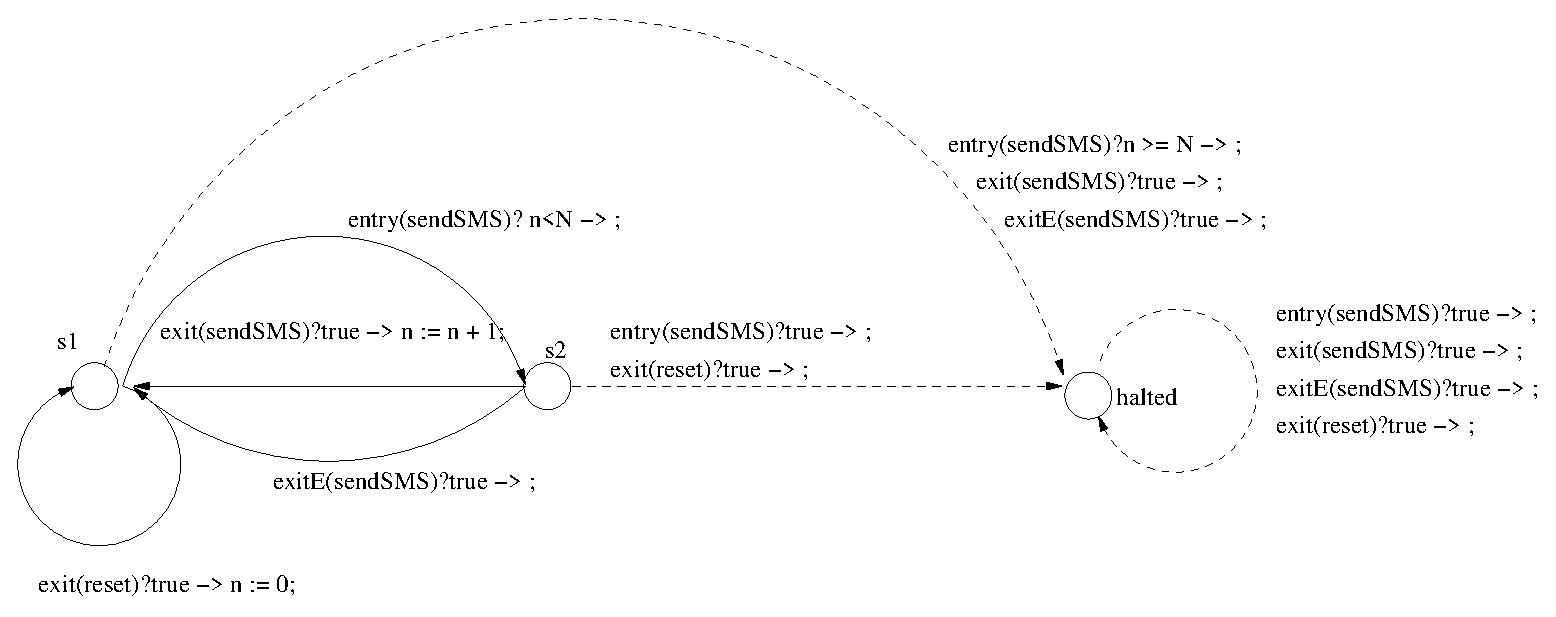
\epsfig{file=complete.eps, width=7cm}
\end{center}
\caption{Automaton of Fig.~\ref{FigExample}, after completion}\label{FigCompletePA}
\end{figure}



\section{Programs and Semantics}\label{SecProgram}

This section first defines an abstract syntax of programs, followed by
their semantics. Both are fairly standard, except that the semantics
is parametrised on the treatment of specifications. In particular, we
define a run-time checking and a monitoring semantics, that evaluate
differently upon method call and exit.


\subsection{Program Syntax}\label{SecSyntax}
Our language is a restricted subset of (sequential) Java, abstracting
away from typical object-oriented features. This means in particular
that we abstract away from method resolution; instead we assume that
the annotated class contains method bodies for the relevant methods,
thus method lookup is trivial. Similarly, we assume that lookup of
class invariants returns the complete class invariant, including those
invariants that are inherited from superclasses. We consider
only a few exceptions, and assume that methods have only one
parameter. We believe, however, that our formalisation contains all
constructs that are relevant for proving correctness of our inlining
algorithm for class-based monitoring, and implementing the
algorithm for the full language is mainly an engineering issue.

\begin{figure}[t]
\[{\small
\begin{array}{rcl}
\Expr & = & \Plus(n_1, n_2 : \Expr) \mid
            \EvalN(n : \Name) \mid
            \Not(b : \Expr) \mid
            \Conj(b_1, b_2 : \Expr) \mid \\
      &   & \Eq(e_1, e_2 : \Expr) \mid
            \EvalB(n : \Name) \mid
            \EvalR(n : \Name) \mid
            \CondExpr(c, e_1, e_2 : \Expr) \mid\\
      &   & \Assign(n : \Name, e : \Expr) \mid
            \Call(o : \Expr, mn : \Name, p : \Expr) \mid
            \Const(v : \Val) \\
\Stmt & = & \Skip \mid
            \Sequence(s_1, s_2 : \Stmt) \mid
            \IfThenElse(c : \Expr, s_1, s_2 : \Stmt) \mid\\
      &   & \While(c : \Expr, s : \Stmt) \mid
            \StmtExpr(e : \Expr) \mid
            \Throw(e : \Excpt) \mid\\
      &   & \TryCatch(t: \Stmt, e : \Excpt, c, f : \Stmt) \mid
            \Set(n : \Name, e : \Expr) \mid\\
      &   & \CaseJML(b : \listof{\Expr \times \Stmt}) \mid
            \Assert(e : \Expr)
\end{array}}
\]
\caption{Abstract syntax of expressions and statements}
\label{FigExprStmt}
\end{figure}

\begin{figure}[t]
\[{\small
\begin{array}{rcl}
\Method & = \opr & \name : \Name,
                   \param : \LocalVarDecl,
                   \lvars : \setof{\LocalVarDecl},
                   \body : \Stmt,\\
        &        & \res : \Expr,
                   \restype : \Type,
                   \pre, \post : \Expr \rightarrow \Expr, \\
        &        & \preset, \postset : \Expr \rightarrow \Stmt,
                   \excset : \Excpt \rightarrow \Stmt \clr \\
\Class & = \opr & \name : \Name,
                  \super : \Name_{\bot},
                  \fields : \setof{\FieldDecl},
                  \methods : \setof{\Method},\\
        &       & \inv : \Expr,
                  \ghostvars : \setof{\FieldDecl} \clr\\
\Program & = \opr & \classes : \setof{\Class} \clr
\end{array}}
\]
\caption{Abstract Syntax for Programs}\label{FigProgram}
\end{figure}


Figure~\ref{FigExprStmt} defines expressions and statements as a
mutually recursive data type (we use the term \emph{body} to denote
either an expression or a statement). Notice that we define several special
language constructs to represent JML annotations: \Set,
to update ghost variables (\emph{i.e.}, specification-only variables),
\CaseJML, to abbreviate a list of conditional ghost variable updates,
and \Assert, to evaluate a condition on the program state. A standard
program semantics ignores these statements, but the annotated program
semantics evaluates them.

Figure~\ref{FigProgram} describes the syntax for methods,
classes and programs. To ensure that every method has an appropriate
return expression, it is part of the method signature.
Furthermore, methods can be annotated with pre- and postconditions, and
classes with invariants. To support our annotation generation
algorithm, we define special annotations called
\(\preset\), \(\postset\) and \(\excset\). These annotations describe
the updates to the ghost variables at method entry, exit and
exceptional exit, respectively.
Pre- and postcondition and the different method specification-level set
annotations have a function type, to allow the use of the method parameter,
the method result or the returned exception, respectively.

A program is said to be \emph{wellformed} if
\begin{inparaenum}[(\itshape i\upshape)]
\item names of fields, local variables and ghost variables are
disjoint and are not reserved words;
\item class names are unique;
\item method names are unique;
\item every variable name that is used is declared; and
\item only ghost variables are the target of \Set statements.
\end{inparaenum}
% (We have stated only the wellformedness conditions necessary for our
% correctness proofs.)


\subsection{Natural Semantics}\label{SecSemantics}
The behaviour of a program is described via a big step semantics. We
closely follow Von Oheimb's formalisation of Java~\cite{Oheimb01},
with simplifications wherever possible, due to our simplified
program syntax. A judgement $\etp{P}{e,\sigma}{v,\sigma'}$ means that the body
$e$ evaluates to $v$, while transforming the state $\sigma$ into $\sigma'$, in
the context of the program \(P\). Note that \(v\) is \One\ for
normally terminating \emph{statements}, while \(v\) is \(\bot\) whenever
evaluation finishes in an exceptional state.

A basic program state \(\Pstate\) is composed of an optional exception
and a store.  The store maps every field and local variable to a
value.

\[
{\small
\begin{array}{rcl}
\Pstate & = \opr & \ex : \Excp_{\bot}, \st : \PStore \clr\\
\PStore & = \opr & \fvs : \Name \mapsto \Val, \lvs : \Name \mapsto \Val \clr
\end{array}}
\]

Since annotated or monitored programs
contain more information than unannotated programs, the
evaluation rules are parametrised with types
\(\FullProgram\) and \(\FullState\). For each instantiation we give
mappings \program and \progstate to the basic program type \Program
and the basic program state \Pstate. Further, we add parameters that
specify the actions that are taken upon method entry or (normal or
exceptional) exit (\gammain, \gammanorm, and \gammaexc, respectively),
and the handling of annotations (\deltaset, \deltaassert, and
\deltacase).  In a standard program semantics, where specifications
are ignored, these are all instantiated with the identity relation.

The evaluation rules are fairly standard, and we refer to Von Oheimb
and the PVS formalisation for more details.  Evaluation
of normally terminating method calls is described by the following rule
(where for
clarity of presentation, we left out several checks that intermediate
states are not exceptional).

%\begin{figure}[t]
\vspace*{-1em}
\[{\small
\begin{array}{c}
\sigma_0.\progstate.\ex = \bot \qquad        % no exception in sigma_0
\etp{P}{o, \sigma_0}{r,\sigma_1} \qquad      % evaluate receiver
\etp{P}{p, \sigma1}{\act, \sigma_2}\\        % evaluate argument
%\sigma_2.\progstate.\ex = \bot \qquad        % no exceptions in sigma_2
r \not= \Null \qquad                         % receiver not null
\md = \lookupmthd(P, r, \mn) \\
\oldlvs = \sigma_2.\progstate.\st.\lvs \quad
\sigma_3 = \updatelvs(\sigma_2, r, \md.\lvars, md.\param, \act) \\
\gammain(P, \md, r, \Const(\act), \sigma_3, \sigma_4) \qquad
\etp{P}{\md.body, \sigma_4}{\One,\sigma_5} \\
\etp{P}{\md.\res, \sigma_5}{v,\sigma_6}\qquad
%\ex(\progstate(\sigma_6)) = \bot
\gammanorm(P, \md, r, \Const(v), \sigma_6, \sigma_7)\\
%\ex(\progstate(\sigma_7)) = \bot\\
\hline
\etp{P}{\Call(o,\mn,p), \sigma_0}{v, \sigma_7
(\progstate.\st.\lvs := \oldlvs)}
\end{array}}
\]
% \caption{Evaluation rule for normal termination of method
% calls}\label{FigEvalRules}
% \end{figure}

First the receiver is evaluated, resulting in non-null reference
\(r\).  Next, the parameter is evaluated, resulting in value
\act. Using \(r\), the method definition
\md is looked up.  The local variable store is updated assigning
\(r\) to \texttt{this}, initialising the method's local variables and
assigning the actual parameter to the formal parameter. The old local
variable store is remembered as \oldlvs.  Next, an appropriate action
upon method entry is taken, as specified by the relation
\(\gammain\). Then the method body, and method result expression are
evaluated. Since this rule applies to normal method termination only,
the parameter for normal method termination \(\gammanorm\) is
evaluated.  Last, the local store is set back to \(\oldlvs\). In
addition, rules exist that specify behaviour of a method call when it
is called upon a null reference, the body contains an uncaught
exception \emph{etc.}


\paragraph{Annotated Program Semantics}

The program state of an annotated program is extended with a store for
ghost variables:
\[{\small
\Astate = \opr \pstate : \Pstate, \gvs : \Name \mapsto \Val \clr}
\]
The types \FullProgram and \Program coincide, while \FullState is
instantiated as \Astate, and the mapping \progstate is defined as
\pstate. Figure~\ref{FigAnnotatedSem} shows some of the
instantiations of the semantics parameters; % (presented in rule format);
the other instantiations are similar. The relation \gammain uses
the auxiliary relation \(\beta\) which checks a boolean expression \(e\) and
raises a special \JMLExc if it evaluates to false. Upon method
entry, the class invariant and precondition are evaluated. If they
fail, a \JMLExc is thrown, otherwise the method's \preset statement is
executed. Finally, we ensure that the program store is not changed.
The function \deltaset updates a ghost variable: it first evaluates the
expression and if this did not result in an exceptional state, it updates the
value of the ghost variable\footnote{We use \(\tau(\gvs.n := v)\) to
abbreviate that the value of \(\gvs(n)\) in \(\tau\) is updated to
\(v\).} appropriately.

%% Relation with the code:
%% r = a, act = arg, \sigma_1 = s1, \sigma_2 = s2, \beta = check_assertion
\begin{figure}[t]
\[{\small
\begin{array}[t]{c}
\invar = \lookupinv(P, r) \qquad
\beta(P, \invar, \sigma_1, \tau_1) \qquad
\beta(P, \md.\pre(\act), \tau_1, \tau_2) \\
\etp{P}{md.\preset(\act), \tau_1}{v,\tau_2} \qquad v\in\{\bot,\One\} \qquad
\sigma_1.\pstate.\st = \sigma_2.\pstate.\st\\
\hline
\gammain(P, \md, r, \act, \sigma_1, \sigma_2)
\smallskip\\


\etp{P}{e, \sigma_1}{v, \tau} \qquad
\pif{v = \B(\ttt)}{\sigma_2 = \tau}{\sigma_2 = \tau (\ex := \JMLExc)}\\
\hline
\beta(P, e, \sigma_1, \sigma_2)

\smallskip\\

\etp{P}{e, \sigma_1}{v, \tau} \qquad
\pif{\tau.\pstate.\ex = \bot}{\sigma_2 = \tau (\gvs.n := v)}{\sigma_2 = \tau}\\
\hline
\deltaset(P, \Set(e, n), \sigma_1, \sigma_2)
\end{array}}
\]
\caption{Instantiation of semantics for runtime annotation evaluation}
\label{FigAnnotatedSem}
\end{figure}


\paragraph{Monitored Program Semantics}
The parametrised program semantics is also instantiated for monitored
programs. This semantics is only defined when the PA is compatible
with the program. PA \(a\) is said to be compatible with a program
\(P\), denoted \(a \sqsubseteq P\), if
\begin{inparaenum}[(\itshape i\upshape)]
\item the program contains the class \(c\) that is being monitored,
\item all variables declared as program variables in
\(a\) are fields of the class \(c\) with the correct type, and
\item every event name corresponds to a method in the class.
\end{inparaenum}
A monitored program is a product of a PA and a program. The state of a
monitored program consists of the states of the PA and the program
(including ghost variables)\footnote{For convenience, we assume that a
monitored program also evaluates annotations, but this instantiation
is in fact orthogonal to the annotated program semantics.}, and a flag
\stuck. If the PA is partial, the flag
\stuck is set when \(\Delta_a\) is not defined for a
certain input. If the flag is set, this means that the security policy
is violated, and the program should be stopped (by some external
observer). If the PA is total, the \stuck flag will never be
set. Instead, violation of the security policy is modelled by the PA
reaching the trap state \halted (in which case the external observer
again is supposed to stop execution).

\vspace*{-1em}
\[
{\small
\begin{array}{rcl}
\Mprogram & =  & \opr \pa : \PA, \program : \Program \clr\\
\Mstate & = & \opr \pastate : \PAstate, \pstate : \Pstate, \gvs :  \Name \mapsto \Val, \stuck
: \BoolSet \clr
\end{array}}
\]
Thus, \FullProgram gets instantiated as \Mprogram and \FullState as
\Mstate, with mappings \program and \pstate. Now we can give
appropriate instantiations for the \(\gamma\)- and
\(\delta\)-relations. The \(\delta\)-relations are the same as
for the annotated program semantics, but the \(\gamma\)-relation also
updates the state of the monitor. For example, \(\gammain\) is defined
in terms of \(\gammain\) for annotated programs, as defined in
Figure~\ref{FigAnnotatedSem}.
\[
{\small
\begin{array}{c}
\gammain^{\mathsf{AP}}(P, \md, r, \act, \sigma_1, \tau) \\
\pif{\tau.\pstate.\ex = \bot}
    {\sigma_2 = \gammapa(\entry)(P, \md, \act, \tau)}
    {\sigma_2 = \tau}\\
\hline
\gammain(P, \md, r, \act, \sigma_1, \sigma_2)
\end{array}}
\]


\noindent where
% NOTE: This is a simplified version of on_method_MVA in MonitoredProgram
\[
{\small
\begin{array}[t]{rcl}
\gammapa(\ev)(P, \md, \act, \sigma) & = &
\begin{array}[t]{l}
\mathsf{let\ }
\begin{array}[t]{rcl}
  e & = & \opri \etype := \ev, \mname := \md.\name \clri\\
 \tau & = & \Delta_{P.\pa}(\sigma.\pastate, \sigma.\progstate, e, \act)
\mathsf{\ in\ }\end{array}
\\
\pif{\sigma.\stuck \vee \tau = \bot}
    {\sigma (\stuck := \ttt)}
    {\sigma (\pastate := \tau)}
\end{array}
\end{array}}
\]

\section{Annotation Generation}\label{SecAnnotGen}

Given a security property encoded as an MVA, the annotation generation
procedure generates JML-annotations that capture this property,
\emph{i.e.}, if the program does not violate the generated % AT: shouldn't be iff?
JML-annotations, it respects the security property encoded by the
MVA. As explained above, the procedure is defined in several steps:
\begin{inparaenum}[(\itshape i\upshape)]
\item the monitor is completed (as described in Section~\ref{SecMVA});
\item the annotations are generated at the method specification level,
as special set-annotations; and
\item the method specification-level set-annotations are inlined in
the method body.
%\item the special \CaseJML construct that is used to make the
%annotations more compact is translated into a sequence of \Set
%annotations.
\end{inparaenum}
%Notice that the order of the last two steps can be swapped.
Notice that the special \CaseJML constructed could be translated into
standard JML annotations as well.

For each step we prove that the old and the new program are bisimilar,
\emph{i.e.}, we show for every translation step
\(\alpha\) there exists a relation \(R\) such that:
\[{\small
\begin{array}{l}
\forall b, \sigma_1, \sigma_2, \tau_1, v_1.
\etp{P}{b,\sigma_1}{v_1, \sigma_2} \wedge
R(\sigma_1, \tau_1) \Rightarrow \\
\qquad
\exists \tau_2, v_2.
\etp{\alpha(P)}{b, \tau_1}{v_2, \tau_2} \wedge
R(\sigma_2, \tau_2)
\end{array}}
\]
and vice versa. Additionally, we show that the initial program states
are related by \(R\), and from this we can conclude that for any
reachable states there exists a related state, reachable in the
translated program.

A natural way to prove this is by induction over the derivation
length. However, to do this, we have to make some restrictions. In
particular, the translation introduces new (ghost) variables to encode
the MVA. Therefore, to be able to apply induction, we typically
require that the body \(b\) does not contain any new variables. The
new variables occur only at specific points in the program, and for
these point separate preservation lemmas have to be proven. Further,
to be able to complete the proof, we need to ensure that in both
bodies the same branches of conditional expressions and statements are
taken, and that the same values get assigned to the store. Therefore,
we prove a stronger result, adding that also the resulting values
\(v_1\) and \(v_2\) are the same (however, sometimes this holds only
under certain conditions).



This section presents more details of the different translation steps,
and presents the relation that witnesses the bisimulation.  Further,
we discuss the special conditions under which the bisimulation holds.

%\begin{figure}
%\begin{center}
%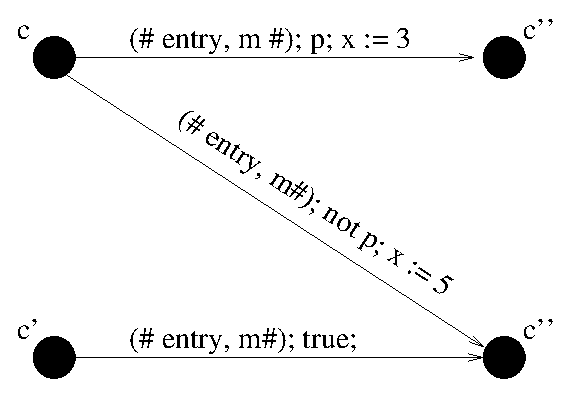
\epsfig{file=annotgen_example, width=4cm}
%\end{center}
%\caption{MVA fragment to illustrate set-annotation
%generation}\label{FigAnnotGenExample}

%\end{figure}

\paragraph{Completion of the automaton}
The first translation step does not change the program itself, it only
completes the MVA. Suppose that \(P\) is a monitored program, where
\(\mva(P)\) is deterministic and wellformed. Then the translation to a
monitored program with a total MVA, \(\alpha_1(P)\), is defined as:
% This is complete_MP in MonitoredProgramCompletessRelation
\[{\small
\alpha_1(P) = \opri \mva := \complete(P.\mva), \program := P.\program
\clri
}
\]

The relation that is preserved between executions of \(P\) and
% This is monitor_related_states
\(\alpha_1(P)\) is the following (where \(\sigma\) is a state of
\(P\) and \(\tau\) is a state of \(\alpha_1(P)\)):
\[{\small
R(\sigma, \tau) =\\
 \begin{array}[t]{l}
  (\pif {\sigma.\stuck}{\tau.\mvastate.\cp = \halted\\\ }
        {\sigma.\mvastate.\cp = \tau.\mvastate.\cp}) \:\wedge \\
  \neg \tau.\stuck \:\wedge\\
  (\sigma.\mvastate.\stA = \tau.\mvastate.\stA) \:\wedge
  (\sigma.\progstate = \tau.\progstate)
\end{array}}
\]
% TODO: should we add the condition on ghost variables?

To prove that this relation is preserved for any body \(b\), we make
use of equivalence (\ref{MVAcompletionProp}) on
Page~\pageref{MVAcompletionProp} and we observe further that
\begin{inparaenum}[(\itshape i\upshape)]
\item if \stuck has been set, it remains set,
\item if the MVA is total and \halted is reached, it is never left, and
\item if the MVA is total, \stuck is never set.
\end{inparaenum} Formally, where \(P\) is a monitored program, and
\(Q\) is a monitored program with total MVA:
\[{\small
\begin{array}[t]{rl}
\sigma_1.\stuck \wedge \etp{P}{b,\sigma_1}{v,\sigma_2} \Rightarrow &
\sigma_2.\stuck \\
\sigma_1.\mvastate.\cp = \halted \wedge
\etp{Q}{b,\sigma_1}{v,\sigma_2} \Rightarrow &
\sigma_2.\mvastate.\cp = \halted \\
\neg \sigma_1.\stuck \wedge \etp{Q}{b,\sigma_1}{v,\sigma_2} \Rightarrow &
\neg \sigma_2.\stuck
\end{array}}
\]

For our running example, applying translation \(\alpha_1\) means that
where class \texttt{Messaging} as shown above was first monitored
with the partial MVA in Figure~\ref{FigExample}, after the translation
it is monitored with the total MVA in Figure~\ref{FigCompleteMVA}.
% TODO AT: for some reason I get Fig 2 here instead of Fig 3.


\paragraph{From MVA to Annotations}

\begin{figure}[t]
\[{\small
\begin{array}{rcl}
\alpha_2(P) & = &\opri \classes :=
\{\alpha_{2, \mathcal{C}}(c, P.\mva) \mid c \in P.\program.\classes\} \clri\\

\alpha_{2,\mathcal{C}}(c, a) & = &
\mathsf{if\ }c.\name \not = a.\clname \mathsf{\ then\ }c\\
&&
\mathsf{else\ }c \:\opri
 \begin{array}[t]{l}
 \gvs := c.\gvs \cup \newgvs(a)\\
 \inv := \Conj(\Not(\Eq(\texttt{cp}, \texttt{halted})), c.\inv)\\
 \methods := \{\alpha_{2,\mathcal{M}}(m, a) \mid m \in c.\methods\} \clri
\end{array}\\
\alpha_{2,\mathcal{M}}(m, a) & = & m \: \opri
  \begin{array}[t]{l}
  \preset := \begin{array}[t]{l}
             m.\preset; \alpha_{2,\mathcal{E}}(\entry, m.\name, a);
             \Assert(\Not(\Eq(\texttt{cp}, \texttt{halted}))),
             \end{array}\\
  \postset := m.\postset; \alpha_{2, \mathcal{E}}(\exit, m.\name, a)\\
  \excset := m.\excset; \alpha_{2, \mathcal{E}}(\excexit, m.\name, a)
  \clri
  \end{array}\\
\alpha_{2, \mathcal{E}}(e, n, a) & = &
  \alpha_{2, \mathcal{T}}(\{t \mid t \in a.\trans \wedge
                                   t.\event = \opri \event := e,
                                                    \mname := m \clri
                           \})\\
\alpha_{2, \mathcal{T}}(ts) & = &
  \CaseJML(
    \{(\begin{array}[t]{l}
       \Eq(\texttt{cp}, \texttt{q}),\\
       \CaseJML(\{(t.\guard, \Set(\texttt{cp}, t.\tcp; t.\action)) \mid
                  t \in ts \wedge t.\scp = \texttt{q}
               \}))\\
    \mid \texttt{q} \in a.\cps
    \})
    \end{array}
\end{array}}
\]
\caption{Formal definition of translation MVA into annotations}
\label{FigMVAtoAnnot}
\end{figure}


Figure~\ref{FigMVAtoAnnot} contains the formal definition of the
second translation step: from MVA to method-level set-annotations.
Given a monitored program \(P\) where \(\mva(P)\) is total,
the annotation generation algorithm \(\alpha_2\) applies
\(\alpha_{2, \mathcal{C}}\) to all classes.
This function checks whether the class is the one being
monitored. If so, appropriate ghost variables are added to the class
using the function \newgvs, that is not formally defined here. Basically
\begin{inparaenum}[(\itshape i\upshape)]
\item for each control point of the automaton, a (final) ghost
variable declaration is generated, initialised to a unique value
(\emph{i.e.}, we assume we have a function \unique that maps each
control point to a unique value);
\item a ghost variable \texttt{cp} is declared, initialised to the
value of the ghost variable representing the initial control point;
\item for each automaton variable declaration, a ghost variable is
declared with corresponding type and initialisation.
\end{inparaenum}
Further, \(\alpha_{2, \mathcal{C}}\) adds the condition that the
current control point should not be halted to the class
invariant\footnote{For readability, we do not explicitly write the
translation from MVA control points to ghost variables.}, and then it
annotates all methods in the class using \(\alpha_{2,
\mathcal{M}}\). For each method in the class, its \preset, \postset
and \excset are extended with updates to the ghost variables encoding
the automaton. In addition, at the end of the \preset, an \Assert
statement is added to verify that the transition did not reach the
\halted state: in that case program execution should terminate
immediately.  Without this \Assert, the invariant violation would only
be detected after the body is executed. To encode the updates to the
ghost variables, first \(\alpha_{2, \mathcal{E}}\) computes the set of
relevant transitions (\emph{i.e.}, those where the event and method
name correspond). For these transitions, a \CaseJML statement is
generated, where the different cases correspond to the current control
point being equal to a control point \texttt{q}, for any
\texttt{q} in the automaton. For each such \texttt{q}, all transitions
where \(t.\scp\) is \texttt{q} are selected and a \CaseJML
statement is generated, testing for each of the transitions whether
the guard holds, and if so, setting the control point \texttt{cp} to
\(t.\tcp\), and executing the actions that correspond to this
transition.
Notice that the order in which the different cases are generated is
not important: since the MVA is total and deterministic there is
always exactly one case that applies.

% Commented out to save space
% For clarity of presentation, we have ignored here that \preset, \postset and
% \excset are actually functions, taking the method parameter, result or
% exception, respectively as input. However, in the PVS formalisation
% this is correctly handled.

The formalisation does not formally discuss how the guard and the
actions are translated into expressions in the programming
language. Instead, we assume that we can translate the guard and the
action expressions into expressions in the programming
language that
\begin{inparaenum}[(\itshape i\upshape)]
\item are wellformed,
\item give the same result,
\item do not have side-effects,
\item do not throw exceptions,
\item do not contain method calls.
\end{inparaenum}
From this we can conclude that in the annotated program, the generated
statements in the \preset can only throw a \JMLExc (because of the
concluding \Assert), while the generated statements in the \postset
and \excset do not throw any exception.

To show correctness of the translation, we show that the following
relation is preserved (where \(P\) is the monitored program,
\(\sigma\) is a state of the monitored program, and \(\tau\) a state
of the annotated program):
\marginnote{Is OK to have both $\pstate$ and $\progstate$?}
% TODO: Review this definition
\[{\small
\begin{array}{rcl}
% This is related_states
R(\sigma, \tau) & = & \neg \sigma.\stuck \:\wedge\\
& & \begin{array}[t]{l}
\mathsf{if\ }\sigma.\mvastate.\cp = \halted
\mathsf{\ then\ }\tau.\pstate.\ex = \JMLExc
\mathsf{\ else\ }S(\sigma, \tau)
\end{array}\\
% This is mp_modeled?
S(\sigma, \tau) & = &
\begin{array}[t]{l}
\unique(\sigma.\mvastate.\cp) = \tau.\pstate.\gvs(\texttt{cp}) \:\wedge\\
(\forall q \in P.\mva.\cps.\ \unique(q) =
\tau.\pstate.\gvs(\texttt{q})) \:\wedge\\
(\forall n \in P.\mva.\vdsA.\ \sigma.\mvastate(n.\name) =
                             \tau.\pstate.\gvs(\texttt{n})) \:\wedge\\
\sigma.\progstate.\pstate = \tau.\progstate.\pstate \:\wedge\\
(\forall n \in P.\ghostvars.\ \sigma.\progstate.\gvs(n) =
\tau.\progstate.\gvs(n))
\end{array}
\end{array}}
\]
This specifies that if the monitor has reached a \halted
control point, then the annotated program must have thrown a
\JMLExc. Otherwise, the state of the annotated program must correctly
model the MVA, \emph{i.e.}\ the current control point is stored in the
ghost variable \texttt{cp}, and all the MVA control points and
variables correspond to ghost variables. Moreover, the values of the
fields have to coincide, just as the values of the ghost variables
that are declared in the program of \(P\). Notice that if an
annotation that is already present in \(P\) throws a \JMLExc,
both the monitored and the annotated program will throw a \JMLExc.
Therefore, we cannot prove that the annotated program throws
a \JMLExc \emph{if and only if} \halted is reached.

To prove that this relation is a preserved, the property is
strengthened with the following property: if the control point is not
\halted, then the derivations also produce the same value. The crucial
part in the proof is of course what happens upon method call and
termination. For example, when a method is called, first the invariant
and the precondition are evaluated. Assuming that \halted is not yet
reached, the new conjunct of the invariant evaluates to true, and then
a simple induction allows to conclude that after evaluation of the
precondition, the states are still related. Then the original \preset
annotations are evaluated, and again the induction hypothesis allows to
conclude that the resulting states are related. Next, the monitored
program makes an MVA transition, and the annotated program executes
the newly generated set annotations, followed by an \Assert to check
whether \halted has been reached. Here we cannot use the induction
hypothesis, but instead we show manually that the relation is
preserved.

Notice that in \postset or \excset we do not have an \Assert
statement. Since the invariant is evaluated immediately after the
set-annotations, the reaching of \halted will be detected
immediately. For this part of the proof it is crucial that
the newly added invariant is evaluated first.

Finally, to be able to complete the proof, we have to make a
restriction on the behaviour of \TryCatch. We follow the Java Language
Specification in describing its behaviour~\cite{GoslingJSB05}. This
means in particular that if the \emph{finally} block in the statement
terminates abnormally (because of an exception, or any other reason
for abrupt completion), this overrides a possible exception thrown in
the \emph{try} or \emph{catch} block. Thus, for example, if \halted
is reached in the \emph{try} block, and hence a \JMLExc is thrown, this
exception might be overwritten by an exception thrown in the
\emph{finally} block (see also~\cite{Huisman08} for a discussion of
this problem), which would mean that the violation of the security
policy is not signalled to the user. To avoid this, we require that
for all \TryCatch statements in the program, if the \emph{try} or
\emph{catch} block can throw a \JMLExc, then the whole statement
should also terminate exceptionally because of a \JMLExc.


%The exact
%algorithm is best illustrated with an example. Suppose that we have
%the MVA displayed in Figure~\ref{FigAnnotGenExample}, where \texttt{x}
%is supposed to be an automaton variable. It has three transitions
%labelled \(\opri \etype := \entry,
%\mname := m\clri\) for some method \(m\). The \preset annotation
%of method \(m\) contains a \CaseJML statement with three branches: the
%first branch tests whether \texttt{cp} has the value of the ghost
%variable representing control point \(c\) and \(p\) holds, the second
%tests whether we are in \(c\) and \(\neg p\) holds \emph{etc.}. Notice
%that the guards are now legal JML expressions, as all MVA variables
%have been mapped into ghost variable declarations. In the first branch
%\texttt{cp} is set to the ghost variable representing
%\(c''\), and the ghost variable \texttt{x} is set to 3. In the second
%branch,  \texttt{cp} is set to \(c'''\) and \texttt{x} to 5, and in
%the last branch (\texttt{cp} = \(c'\)) \texttt{cp} is always set to
%\(c'''\) and \texttt{x} is not changed.

To illustrate the translation on our running example, consider again
the implementation of the class \texttt{Messaging} and the completed
MVA, encoding the \emph{limited SMS} security policy, in
% TODO AT: again here I get Figure 2
Figure~\ref{FigCompleteMVA}. Figure~\ref{FigExampleStep2} shows the
generated annotations that result from applying translation
\(\alpha_2\) on this program and this MVA. Notice that for methods
and events that are not involved in the property, an empty \CaseJML is
generated~--~this is equivalent to an \Skip statement.

\marginnote{\small There are many vars not declared: s1, s2, halted, N.
Is it just to save space? Should we add some ... in the declarations?
Also cp must be initialized to s1. I added them but in JML we cannot have
two annotations on the same line.}
\begin{figure}[t]
{\small\begin{verbatim}
class Messaging {
  //@ ghost int s1=1; //@ghost int s2=2; //@ghost int N=5;
  int counter; //@ ghost int cp = s1; //@ ghost int n;

  /*@ pre_set  CaseSet [(cp == s1, CaseSet [(n < N, cp = s2),
                                            (n >= N, cp = halted)]),
                        (cp == s2, CaseSet [(true, cp = halted)]),
                        (cp == halted, CaseSet [(true, cp = halted)])];
      post_set CaseSet [(cp == s1, CaseSet [(true, cp = halted)]),
                        (cp == s2, CaseSet [(true, cp = s1; n = n + 1)]),
                        (cp == halted, CaseSet [(true, cp = halted)])];
      exc_set  CaseSet [(cp == s1, CaseSet [(true, cp = halted)]),
                        (cp == s2, CaseSet [(true, cp = s1)]),
                        (cp == halted, CaseSet [(true, cp = halted)])]; @*/
  void sendSMS(){ /* body sendSMS */}

  /*@ pre_set  CaseSet []; post_set CaseSet []; exc_set  CaseSet []; @*/
  void receiveSMS(){ /* body receiveSMS */}

  /*@ pre_set  CaseSet []; exc_set CaseSet [];
      post_set CaseSet [(cp == s1, CaseSet [(true, cp = s1)]),
                        (cp == s2, CaseSet [(true, cp = halted)]),
                        (cp == halted, CaseSet [(true, cp = halted)])]; @*/
  void reset() { /* body reset */}
}
\end{verbatim}}
\caption{Set annotations generated for class Messaging}\label{FigExampleStep2}
\end{figure}



\paragraph{Inlining the Annotations}

Once the set-annotations at method specification level are generated,
the next step is to inline these into the method bodies.  The main
idea is that to ensure that the appropriate set-statements are
executed at the end of the method body, the body is wrapped in a
\TryCatch statement. The translation \(\alpha_3\) applies
\(\alpha_{3, \mathcal{C}}\) to all classes, which in turn applies
\(\alpha_{3, \mathcal{M}}\) to all methods in the class. This function
generates one new local variable\footnote{In fact, this should be a
local \emph{ghost} variable, but as these are not yet supported by our
formalisation, we formalise it as a standard local variable.}
\resl. The body of the method is changed as follows: first \preset is
executed. Then the body of the method is wrapped in two \TryCatch
statements, to catch \Throwable and \NullPointer
exceptions\footnote{For simplicity, we do not model the exception
hierarchy and thus \TryCatch can only catch a single exception, but in
practice only one \emph{try-catch-finally} block would be needed.}.  After
the body is executed (inside the \emph{try} block) the result
expression from the original body is evaluated, and assigned to
\resl. Next, the \postset instruction is executed. Notice that these
are only executed if the body actually terminates normally, otherwise
the exception will simply be propagated. Finally, in the \emph{catch}
clauses, the \excset is executed. The result expression of the method
is the look up of the variable \resl. To conclude, \preset,
\postset and
\excset in the method specification are set to
\Skip. Figure~\ref{FigInline} gives the formal definition of
\(\alpha_{3, \mathcal{M}}\) (where \(P\) is a program, and \(m\) a method).

\begin{figure}[t]
\[
\alpha_{3, \mathcal{M}}(P, m) = m \opri
\begin{array}[t]{l}
\preset := \Skip, \postset := \Skip, \excset := \Skip,\\
\lvars := \{\resl\} \cup m.\lvars,
\res := \lookup(\resl), \\
\body :=
\begin{array}[t]{l}
\TryCatch(\\
\quad \begin{array}[t]{l}
  \TryCatch(
  \begin{array}[t]{l}
   m.\preset; m.\body; \\ \Assign(\resl, m.\res); m.\postset\\
  \end{array}\\
  \Throwable, m.\excset, \Skip),
\end{array}\\
\NullPointer, m.\excset, \Skip) \clri
\end{array}
\end{array}
\]
\caption{Formal definition of annotation inlining for methods}\label{FigInline}
\end{figure}


To prove correctness of this translation, we use the following
relation: all fields and ghost variables coincide, exceptions
coincide, and all local variables that are declared in the original
program coincide. In the correctness proof, we use that the \postset
and \excset annotations do not throw any exceptions, and \preset may only
throw a \JMLExc. Moreover, we use that the set-annotations do not
contain method calls, from which we can conclude that they do not
modify any variables that are not explicitly mentioned in them. In
particular, this allows to conclude that the new local variable is
not changed by the set annotations.

\marginnote{MH: We could show the inlining on the running example, but
this is not very interesting. Since we did not give method bodies, it
will just stay as abstract. AT: I agree}

\section{Related Work}\label{SecRelated}
Cheon, Aktug \& Gurov...

\section{Conclusions and Related Work}\label{SecConcl}

This paper presents the Bytecode Modeling Language (BML). BML allows
one to specify and verify an application directly at the level of
bytecode. Its syntax and semantics are directly inspired by the source
code level specification language JML.  The possibility to reason
direct at the level of bytecode, without relying on a compiler, is of
major importance for guaranteeing the security of applications (for
example in a context of mobile code, where some applications are
written in bytecode directly, to avoid security problems related with
compilation). However, to make such verifications tractable, it is
important that the specification language is intuitive and provides a
sufficient degree of abstraction, without the need to talk too much
about the internal structure of the state (heap, store
\emph{etc.}). BML does exactly this: it is designed to be close to the
source code level specification language JML and provides a high level
of abstraction. It is designed for program verification, and its
semantics supports the development of a verification condition
generator for unstructured code. Moreover, because of its close
connection with JML, it is not too complicated to compile source code
level specification into bytecode level specifications.  The BML
language as we have defined it now, corresponds roughly to JML level
0, \emph{i.e.}\ that part of JML whose semantics is relatively well
understood. However, more advanced constructs of JML can be easily
added to BML, if required.

\begin{figure}[t]
\begin{center}
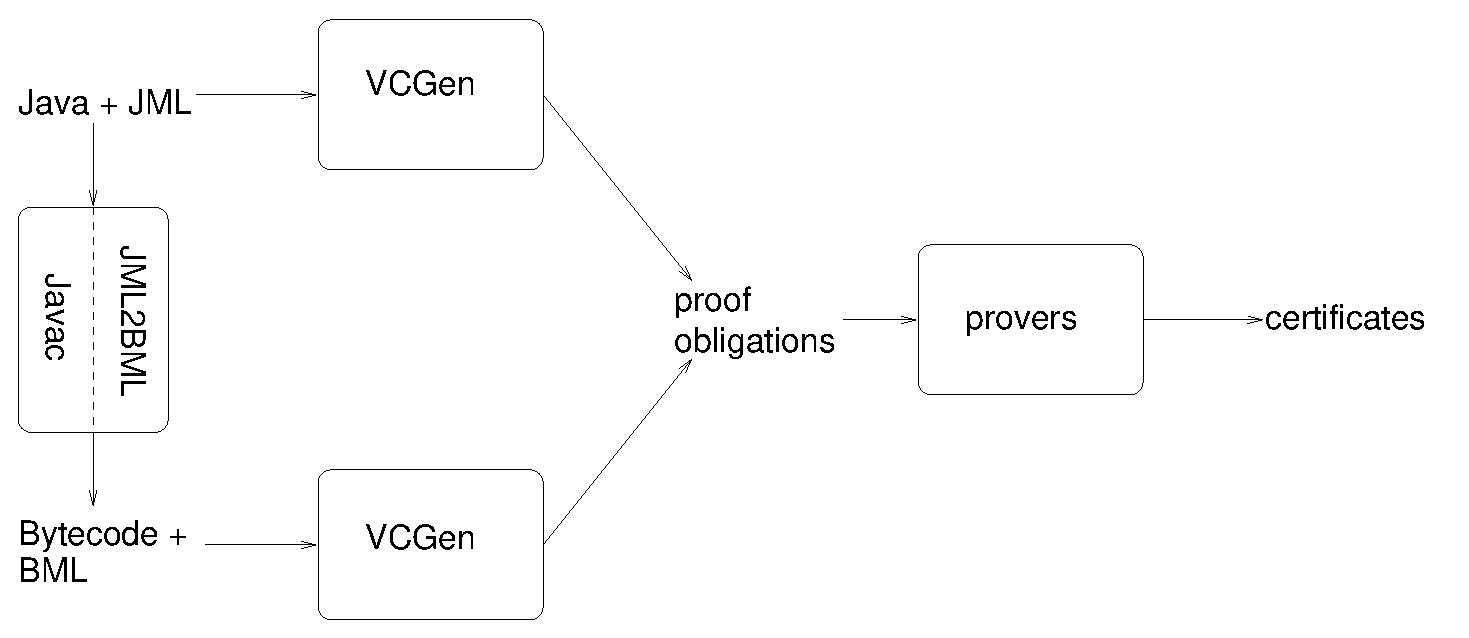
\includegraphics[width=0.8\textwidth]{toolset.eps} 
\vspace*{-1em}
\caption{Overview of \mobius tool set}\label{FigToolSet}
\end{center}
\end{figure}
\paragraph{Tool support}
As part of the \mobius project, we plan to develop a program
verification tool set that supports both JML and
BML. Figure~\ref{FigToolSet} outlines the general architecture of this
tool set. Thus, both Java/JML and bytecode/BML can be used as input
application. Annotated programs are translated into a guarded
command format, for which an appropriate verification condition
generator is used to generate proof obligations that can be discharged
with a theorem prover (either automatic or interactive). To support
the PCC platform, the provers will be instrumented to produce
certificates. In addition, source code applications annotated with JML
can be compiled into bytecode annotated with BML.

The development of the JML subcomponent of the tool set will be based
on experiences with ESC/Java~\cite{CokK04} and JACK~\cite{BurdyRL03}.
Several tools and algorithms (notably the compiler and the
verification condition generator) for BML have already been
implemented, see~\cite{BP06JSV,Pavlova:phd}, but more work is needed
to cover the whole language. Moreover, to make the tool set usable in
practice, we will also need a tool to inspect and write BML
specifications directly, and a run-time checker for BML
specifications. The latter can be implemented by a code
transformation, inserting explicit run-time checks in the bytecode, or
by extending the virtual machine to take the user-specific attributes
with specifications into account.  It is also important to have tool
support for checking the structural and typing constraints for BML
specifications. Such a tool can be built as an extension the Java
bytecode verifier.

Our initial experiments with compilation of specifications has shown
that there exists indeed a correspondence between the proof
obligations generated at source and at bytecode level, modulo
differences in elimination of trivial goals, handling of boolean
expressions, and the naming convention of generated
variables~\cite{Pavlova:phd}. Moreover, when the proofs are done with
the Coq prover, different names are generated for hypotheses at source
code and bytecode level. It is future work to clean up the
compilation, so there is a one-to-one correspondence.




 

\paragraph{Related work}
The interest in specification and verification of bytecode
applications is quite recent, and not too much work has been done in
that direction. Several logics have been developed to reason about
bytecode, \emph{e.g.}~by Bannwart \& M\"uller~\cite{BannwartMueller05}
and within the MRG project~\cite{AspinallEtAl:TPHOLs2004}. However, in
this work the main focus was the development of a sound proof system,
while the focus of BML is to write understandable specifications for
bytecode. JVer is a tool to verify annotated
bytecode~\cite{ChanderEILN05}. However, as specification language they
use a subset of JML, \emph{i.e.}\ a source code level specification language.

The development of BML is clearly inspired by the development of the
JML specification language~\cite{JMLReferenceManual05}. Both JML and
BML follow the Design by Contract principle introduced first in
Eiffel~\cite{Meyer97}. The Boogie project~\cite{BarnettCDJL05}
introduces in similarly the Design by Contract principles into the C\#
programming language, both at source code level and for CIL, the .NET
intermediate language.  The possibility to check a property at
run-time, using the \texttt{assert} construct, has been long 
adopted in the C programming language and recently also in Java (Java
1.5, see \cite[\S 14.10]{JLS}). 

Finally, we should mention the Extended Virtual Platform
project\footnote{See
\url{http://www.cs.usm.maine.edu/~mroyer/xvp/}.}. This project aims at
developing a framework that allows to compile JML annotations, to
allow run-time checking~\cite{AlagicXVP05}. However, in contrast to
our work, they do not intend to do static verification of bytecode
programs. Moreover, their platform takes JML-annotated source code
files as starting point, so it is not possible to annotate bytecode
applications directly.

\vspace*{-.5em}
\subsubsection*{Acknowledgements}
We thank Lennart Beringer and Olha Shkaravska for discussions about
the semantics of BML. 
%\vspace*{-.5em}


\bibliographystyle{plain}
\bibliography{bibli,../specification,everest,crossrefs,strings}

\end{document}
